%!TEX root = ../../report.tex
\chapter{Mathematical model of RuBi} % (fold)
\label{cha:mathematical_model}

The motivation to start the development of the mathematical model was the seek of a set of equations with which calculating the requirements for the actuators could be easily achievable.
\todo{Rewrite this}
This task finally evolved towards the creation of a small toolbox that can be extended to the creation of classic control algorithms based on the robot mathematical model.
The main goal was to compute the values of the necessary parameters to select joint actuators able to keep up with the requirements of the application.
However, by definition, to do so the application needed to be defined to the extent that these dimensions could be obtained.
Thus, this chapter contains the definition of the task Rubi is expected to be able to perform, the control model defined for it and an explanation of the assumptions made in order to simplify the resulting model. 
After, the necessary kinematic model of the robot is presented as an intermediary step to compute the simplified dynamic model of the robot, which is introduced next to it.
All the algorithms described in this chapter have been implemented in MATLAB and can be found in appendix. \ref{}. \todo{add Matlab apendix}

\section{Actuators}
\label{sec_actuators}
%!TEX root = ../../../report.tex

\section{Analysis of vertical jump} % (fold)
\label{sec:jumping_case}
Modeling the dynamics of walking gaits in a bipedal robot with 6 DOF has proved significantly complex and time consuming, even for the planar case.
However, it is essential for the obtainment of the most extreme torque and velocity values to apply to each joint during the motion, necessary to gauge the required actuators for the application.
In order to ease the task, instead of calculating the motion equations for the walking or running cases, it was resolved to model the dynamics of the vertical jump case.
This was decided under the assumption that a structure able to perform a static, vertical jump of a certain height $h$ and determined characteristics on one leg could be able to fulfill the power requirements necessary for running, both from an actuation and a structural point of view.
This assumption was built upon the findings introduced in \cite{jump-run1} and \cite{jump-run2}.

\subsubsection{Vertical jump dynamics} % (fold)
\label{ssub:static_jumping_dynamics}
As explained in section \ref{sec:dimensions}, the dimensions of the robot and its parameters have been conceived to imitate human characteristics and capabilities.
Therefore the jump analysis here will be carried out in resemblance of the human case, based on \cite{jump-dynamics1} and aiming at applying the results to a robot platform, as in \cite{jump-dynamics2}.
The jump case analyzed here can be described according to \cite{jump-dynamics1} as a static, squat jump over one foot with take-off and without counter-movement (SJ-NAS).
Three assumptions have been made regarding the bodies in contact during the landing phase of the robot:

\begin{itemize}
    \item No slipping occurs
    \item Absence rebounding 
    \item There are no structural deformations 
\end{itemize}

The whole jump cycle has been divided into two phases with different analysis: an impulse and an aerial period.

\begin{figure}[ht!]
    \centeringx
    \begin{subfigure}[b]{0.3\textwidth}
        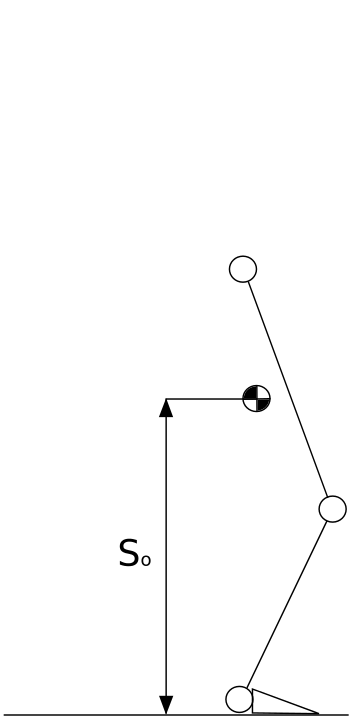
\includegraphics[width=\textwidth]{figures/launch_phase.png}
        \caption{Launch phase}
        \label{fig:launch_phase}
    \end{subfigure}
    \begin{subfigure}[b]{0.3\textwidth}
        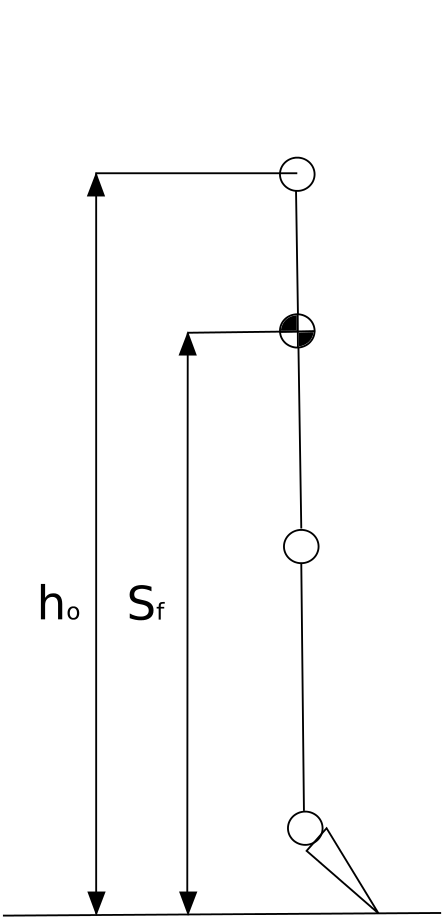
\includegraphics[width=\textwidth]{figures/takeoff_phase.png}
        \caption{Takeoff phase}
        \label{fig:takeoff_phase}
    \end{subfigure}
    \begin{subfigure}[b]{0.3\textwidth}
        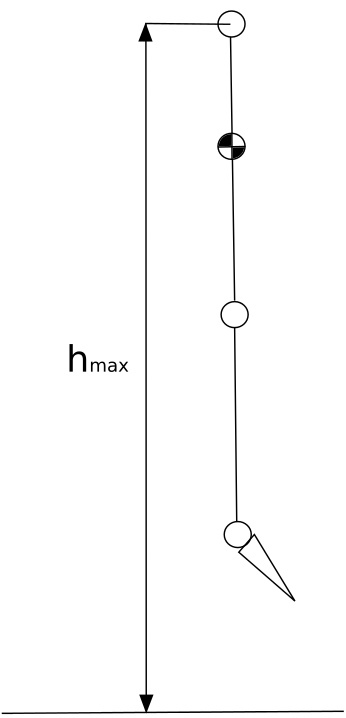
\includegraphics[width=\textwidth]{figures/flight_phase.png}
        \caption{Aerial phase}
        \label{fig:aerial_phase}
    \end{subfigure}
    \caption{Jump phases without fall and landing}
    \label{fig:jump_phases}
\end{figure}


\paragraph{The aerial phase}
The period from the take-off of the toes to the instant in which the maximum height $h_{max}$ has been reached, which can takes place between the instants represented in \ref{fig:takeoff_phase} and \ref{fig:aerial_phase}. 
The rest of the cycle, including fall and landing are not described here.
During the whole period the robot is considered a rigid solid.
This phase is analyzed following the equations of a static projectile motion for the vertical launch case, expressed in \ref{eq:vertical_motion} and \ref{eq:vertical_energy}.

%\begin{equation}
%\label{eq:vertical_motion}	
%	h(t) = V_o t sin(\theta) - \cfrac{1}{2} g t^2 
%\end{equation}

\begin{equation}
\label{eq:vertical_energy}
	m g \Delta h = \cfrac{1}{2} m \Delta V^2
\end{equation}

The equation \ref{eq:vertical_energy} is an energy balance analysis for the flight phase, that can be rearranged as showed in \ref{eq:deltaV}

\begin{equation}
\label{eq:deltaV}
	\Delta V = \sqrt{2 g \Delta h}
\end{equation}

This equation can be used to input the desired displacement in the CoG of the robot during the free flight period and obtain the necessary velocity at take-off $V_{toff}$, which is the one the robot has to reach in the impulse phase.
This can be done since $V_{final} = 0$ and therefore $\Delta V = V_{toff}$.

\paragraph{The impulse phase}
From the initial position at the beginning of the jump, depicted in \ref{fig:launch_phase}, to the instant when the toes of the standing foot take off the ground and the ground reaction force ceases, shown in \ref{fig:takeoff_phase}.
The change in momentum in the robot, of mass $m$, caused by the application of a vertical force with the foot to the ground $F$ during a period $t$ is given by equation \ref{eq:impulse}, derived from the second law of motion of Newton.

\begin{equation}
\label{eq:impulse}
	F  t = m  \Delta V	
\end{equation} 

Substituting equation \ref{eq:deltaV} in \ref{eq:impulse}, the necessary impulse to reach the desired maximum height can be computed.
However, since the force applied to the mass and the application period cannot be decoupled from the result of the equation, an energy analysis has to be carried out together with a posterior optimization of the two values for the desired design of the robot.
Solving equation \ref{eq:impulse} for a small range of application time values and after computing \ref{eq:deltaV} with increasing values of $\Delta h$ in the range $[0.01,0.1]$ meters yields a reciprocal graph whose positive quadrant can be seen in Figure \ref{fig:f-t}

\begin{figure}[ht!]
	\centering
	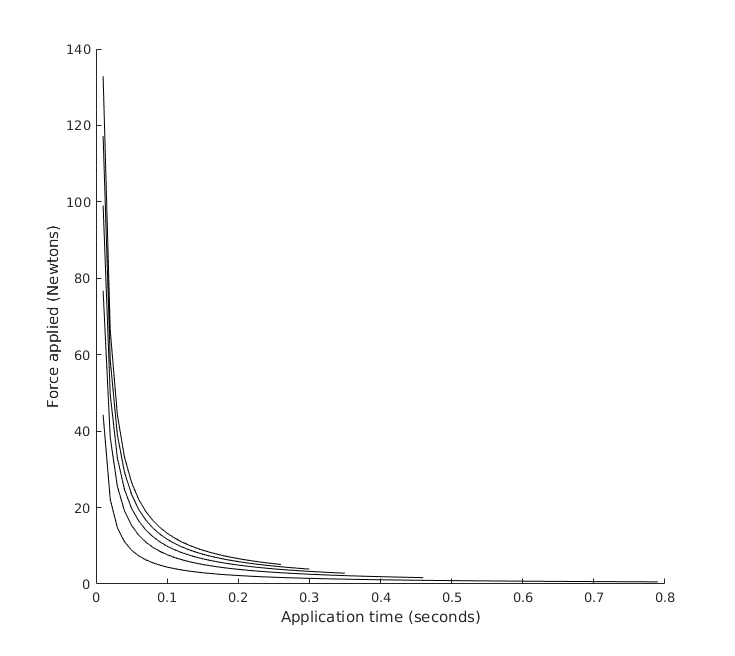
\includegraphics[width=0.8\textwidth]{figures/force-timePlot.png}
	\caption{Force-application time values for the same work magnitude}
	\label{fig:f-t}
\end{figure}

However, the obtained graphs do not propagate to an infinite value of application time, existing a boundary farther than which, the impulse will not produce enough variation in the momentum to launch the body.

\begin{equation}
\label{eq:work}
	W = \int_{t_{toff}}^{t_{f}} F(t)\,\mathrm{d}t = \cfrac{1}{2} m \Delta V^2 = F_{min} S
\end{equation}

Equation \ref{eq:work} describes how the work performed by the robot during the impulse phase can relate to the change in its kinetics energy. 
This equation, derived also from Newton's second law would only apply to rigid bodies without internal degrees of freedom, which is not the case.
However, it has been assumed that the displacement given by $S$ is the vertical translation of the CoM of the robot during the impulse and that it is small enough to be a valid assumption in order to use this procedure.
From Figure \ref{fig:jump_phases}, the displacement of the CoM during the impulse is given as $S=S_{f}-S_{o}$.
Knowing the value of $S$, the minimum necessary force can be obtained, and hence its corresponding application time on Figure \ref{fig:f-t} for a given $\Delta h$.
The displacement of the CoM, $S$ will depend on the initial configuration of the robot prior starting the impulse, and its final one.
Furthermore, for a given $\Delta h$, a range of possible values of the ground reaction Force $F$ can be computed within the limits established and a time can be obtained.
Thus, for a determined $\Delta h$ and $t$ values, a $F$ has to be applied by the foot again the ground.
In order to translate that force to joint effort, the dynamic model of the robot is required.

% subsubsection static_jumping_dynamics (end)

% section The_jumping_case (end)
%!TEX root= ../../../report.tex

\section{Kinematic model}
\label{sec_kinematic_model}
The kinematics model of the robot describes the motion of every joint in time disregarding dynamic parameters.
It is used here to compute position, velocity and acceleration of the limbs for given trajectories of the toes, which are the contact point with the ground in the presented study case, through their forward kinematics.
Also the inverse kinematic model is constructed as a tool for the posterior computation of the dynamics model and its application to model the necessary actuators.
The model has been obtained through direct application of trigonometry instead of using the D-H parameters given its simplicity.
To do so, as explained before the case has been reduced to a two-dimensional study of one leg, where each robot leg haS been analyzed as a kinematic chain of three degrees of freedom.
The main reference frame has been placed attached to the hip with its Y axis parallel to the ground, as if this was the base of a robotic arm, and the toe was the tool, has shown in Figure \ref{fig:kinematics}.
This representation has been chosen to ease the construction of the mathematical model.

%%add world reference frame attached to the ground for flight phase study
\begin{figure}[ht]
	\centering
	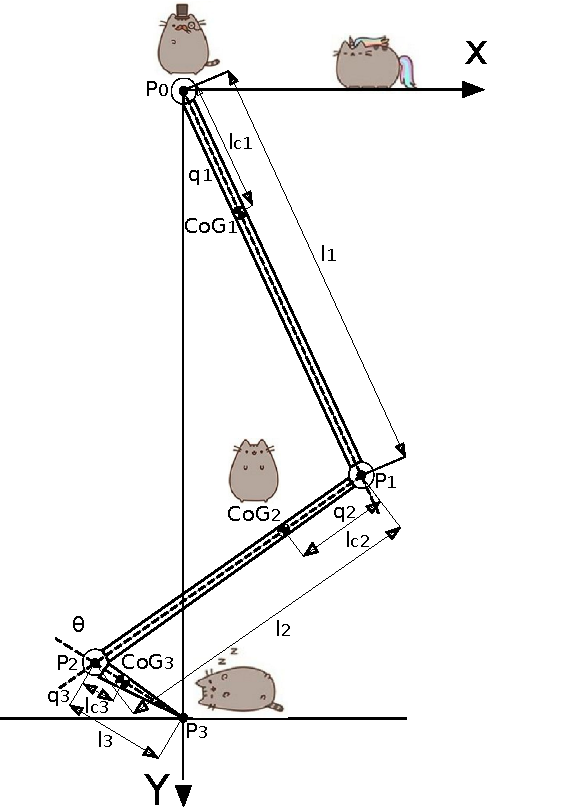
\includegraphics[width=0.4\textwidth]{figures/kinematics_model_kitties.pdf}
	\caption{Coordinate definitions for the schematic model of one leg}
	\label{fig:kinematics}
\end{figure}

The figure above depicts the schematic representation of only one leg, since the other one is equivalent. 
The system is said to be in single support phase since there would be just one foot in contact to the ground.
In the analyzed case, the swinging leg (not represented in Figure \ref{fig:kinematics}) would be static and could be considered an additional link with no degrees of freedom.
The variables $q_{i}$ represent the angles of the joints with respect to their fully-stretched positions to simplify the obtainment of the forward kinematic model, while the angle $\Theta$ is used to express the orientation of the ankle in an absolute manner. 
From Figure \ref{fig:kinematics}, the forward kinematic model in \ref{eq:forward_kinematics} can be easily obtained.


\begin{equation}
\label{eq:forward_kinematics}
	\begin{aligned}
		x_{0} &= 0 \\
		y_{0} &= 0 \\
		x_{1} &= l_{1} \sin(q_{1}) \\
		y_{1} &= l_{1} \cos(q_{1}) \\
		x_{2} &= l_{1} \sin(q_{1}) + l_{2} \sin(q_{1}+q_{2}) \\
		y_{2} &= l_{1} \cos(q_{1}) + l_{2} \cos(q_{1}+q_{2}) \\
		x_{3} &= l_{1} \sin(q_{1}) + l_{2} \sin(q_{1}+q_{2}) + l_{3} \sin(q_{1}+q_{2}+q_{3}) \\
		y_{3} &= l_{1} \cos(q_{1}) + l_{2} \cos(q_{1}+q_{2}) + l_{3} \cos(q_{1}+q_{2}+q_{3}) 
	\end{aligned}
\end{equation}

The variables $x_{i}, y_{i}$ represent the position coordinates of the joints in the right leg, named $P_{i}$ in the schematic in Figure \ref{fig:kinematics} and $P'_{i}$ for the left leg (not depicted).
Once computed, the linear velocity and acceleration of every joint can be obtained by derivation of the forward kinematic model and represented as $\dot{P}_{i}$ and $\ddot{P}_{i}$.

%Add space state vector

The model presented is the most basic one and does not contain the degrees of freedom that could be introduced by springs in the actuators.
This is due to two reasons:

\begin{itemize}
	\item Their configuration can be changed to series, parallel or none in both knees and ankles.
	\item The study of the jump case regarding the parameterization of the actuators has been carried out in the most disadvantageous scenario from the energetic point of view, which in this case means no springs.
\end{itemize}

Following the same approach, the inverse kinematic model can be computed for the right leg, yielding equation \ref{eq:inverse_kinematics}.


\begin{equation}
\label{eq:inverse_kinematics}
	\begin{aligned}
		x_{2} &= x_{3} - l_{3} \sin(\Theta) \\
		y_{2} &= y_{3} - l_{3} \cos(\Theta) \\
		q_{1} &= \arctan \left(\frac{x_{2}}{y_{2}}\right) - \arccos \left(\frac{x_{2}^2 + y_{2}^2 + l_{1}^2 - l_{2}^2}{2 l_{1} \sqrt{x_{2}^2 + y_{2}^2}}\right) \\
		q_{2} &= \pi - \arccos \left(\frac{l_{1}^2 + l_{2}^2 - x_{2} - y_{2}}{2 l_{1} l_{2}}\right) \\
		q_{3} &= \Theta - q_{1} - q_{2} \\
	\end{aligned}
\end{equation}

And equivalently to the forward kinematics, the inverse kinematic model can be derived to obtain the velocities and accelerations in the joint space $\dot{q_{i}}$ and $\ddot{q_{i}}$.

%!TEX root= ../../../report.tex
\section{Dynamic model}
\label{sec_dynamic_model}
The goal of this step is to calculate the relationship between an external force applied to the toe (ground reaction force while jumping) and the necessary torques in the joints for dealing with that external disruption.
This relation can be expressed as a set of second order differential equations represented for the general case as in equation \ref{eq:dynamics_eq1}. 

\begin{equation}
	\label{eq:dynamics_eq1}
	B(q)\ddot{q} + C(q,\dot{q})\dot{q} + g(q) = \tau
\end{equation}

Where $B(q)$ is the inertia matrix, $c(q,\dot{q})$ contains the centrifugal and coriolis acceleration terms and $g(q)$ represents gravity, as in \cite{dynamics1} and \cite{dynamics2}. 
It must be remarked here that the constructed model does not introduce joint friction terms.
For an open kinematic chain as this, three methodologies to obtain the above equation where object of study:

\begin{itemize}
	\item A simplified Euler-Lagrange algorithm, as introduced in \cite{E-L1}, which makes use of the Lagrangian formulation to describe the behavior of the system through work and energy.
	\item The so called Energy Method, presented in \cite{asada} and consisting in finding the relation between the force in the end-effector and the joint torques through the Jacobian of the kinematic chain.
	\item The Newton-Euler algorithm, through which the dynamics of the system can be expressed in terms of forces and moments applied in each member of the chain.
\end{itemize}

It was finally decided to apply the third option due to the fact that it was faster to implement than the E-L algorithm and more reliable than the Energy method.
The Newton-Euler algorithm is founded in classical mechanics and its a recursive method that computes in two steps the velocities and accelerations of every component of a kinematic chain and their forces and torques on the joints.
In \ref{eq:N-E_eq1}, the equations of motion for an individual link are shown.

\begin{equation}
\label{eq:N-E_eq1}
	\begin{aligned}
		f_{i-1, i} - f_{i,i+1} + m_{i} g - m{i} \dot{V}_{ci} =& 0 \\
		N_{i - 1 , i} - N_{i , i + 1} - ( r_{i - 1 , i} + r_{i , Ci} ) \times f_{i - 1 , i} + ( - r_{i , Ci} ) \times ( - f_{i , i + 1}) - I_{i} \dot{\omega_{i}} - \omega_{i} \times ( I_{i} \omega_{i} ) =& 0 \\
		i = 1,..., N 
	\end{aligned}
\end{equation}

These equations contain the coupling forces and moments applied to the link by the immediate ones, however, they cannot be used with them. 
$\omega_{i}$ and $\dot{\omega_{i}}$ represent respectively the angular velocity and acceleration vectors of link $i$ and can be obtained from the joint velocities and accelerations, computed in the previous section, as in equation \ref{eq:angular_magnitudes}.
$I_{i}$ are the inertia matrices of the links, calculated in SolidWorks for the final design of Rubi.

\begin{equation}
\label{eq:angular_magnitudes}	
	\begin{aligned}
		\omega_{i} &= \omega_{i-1} + \xi_{i}\dot{q}_{i}Z_{base}^i\\
		\dot{\omega_{i}} &= \dot{\omega_{i-1}} + \xi_{i}[\ddot{q}_{i}Z_{base}^i + \dot{q}_{i}\omega_{i-1} \times Z_{base}^i]
	\end{aligned}
\end{equation}

The closed-form equations must be derived from them so that they can be applied to the algorithm.
This is done by substituting the coupling forces in the final set of 6 equations obtained for $N=3$ and substituting \ref{eq:torques} in the resulting equations.

\begin{equation}
\label{eq:torques}
	N_{i - 1 , i} = \tau_{i}
\end{equation}

Equation \ref{eq:torques} is valid only for the planar case.
After these steps, a set of three equations of the form \ref{eq:dynamics_eq1} is obtained. 
As parameters, they contain the masses of the links, their vectorial positions, the gravity term and their inertia matrices. 

\todo{add final motion equations?}

This set of equations calculates the necessary torques on the joints as a function of the joints displacements and the external forces and torques applied on the system, as represented in \ref{eq:tau_q}.

\begin{equation}
\label{eq:tau_q}
	\tau(t)_{i} = f(q_{i}(t), \dot{q}_{i}(t), \ddot{q}_{i}(t), \tau_{ext}, F_{ext})
\end{equation}

However, in order to use it the functions that model the trajectories of joints in the joint space must be approximated.
For the ideal static, vertical jump case under study here, the movement of the toe has been constrained to a vertical displacement along the $Y$ axis in order to simplify this task.
Thus, the trajectory of the end-effector of the kinematic chain, $P_{3}$ in Figure \ref{fig:f-t}, can be easily approximated as a function of the form shown in 

\begin{equation}
\label{eq:toe_trajectory}
	\begin{aligned}
	x_{3}(t) &= 0 \\
	y_{3}(t) &= Y_{3}(t_{o}) + \cfrac{Y_{3}(t_{f}) - Y_{3}(t_{o})}{(t_{f} - t_{o}) (t - t_{o})} \\
    \theta(t) &= \theta(t_{o}) + \cfrac{\theta(t_{f}) - \theta(t_{o})}{(t_{f} - t_{o}) (t - t_{o})} 
    \end{aligned}
\end{equation}

Therefore, if equation \ref{eq:toe_trajectory} is used as the input to the inverse kinematic model, the joint displacements will become dependent on the linear displacement of $P_{3}$, and equations \ref{eq:tau_q} will be rewritten as \ref{eq:tau_p}.

\begin{equation}
\label{eq:tau_p}
	\tau(t)_{i} = f(P_{3}(t), \tau_{ext}, F_{ext})
\end{equation}






%!TEX root= ../../../report.tex

\section{Springs influence in the actuators}
\label{sec_springs}
This section deals with the calculations carried out in order to model the influence of the implemented compliance in terms of energy efficiency and joint torque requirements.
As explained in \ref{sec:joints}, the selection of the elastic actuators installed and their configuration on RuBi has been left as a customizable feature for research purposes.
This, together with the fact that RuBi has not been designed to optimize a specific type of gait made pointless the calculation of optimal values of springs.
Thus, the following is just a theoretical frame presented to provide an easy method to compute the influence of the springs in the performance once the user has selected them.
It was meant to be used for the experiments devised on compliance influence in hopping motion, presented in \ref{cha:experiments}.

\subsection{Torque and energy contribution of passive actuators} % (fold)
\label{sub:torque_contribution_of_passive_actuators}
All the springs that can be implemented in RuBi are torsional, as shown in \ref{sub:spring_integration}, whose general equations for torque and energy storage are shown in \ref{eq:torsion_spring}. 

\begin{equation}
\label{eq:torsion_spring}
\begin{aligned}
	\tau_{S} &= -K \Delta \theta \\
	U_{S} &= \frac{1}{2}K \Delta \theta^2
\end{aligned}
\end{equation}

The contribution of the springs torques to the system actuation is therefore modeled introducing the torque equation in \ref{eq:torsion_spring} on the right side of \ref{eq:dynamics_eq1}, which would yield equation \ref{eq:dynamics_eq2}.
Where the torques vector has been divided into the motors and springs inputs.

\begin{equation}
	\label{eq:dynamics_eq2}
	B(q)\ddot{q} + C(q,\dot{q})\dot{q} + g(q) = \tau_{M} + \tau_{S}
\end{equation}

The values of $\Delta \theta_{i}$ can be obtained through forward kinematics for given trajectories, while $\tau_{i}$ can be computed from equation \ref{eq:dynamics_eq1} given the ground contact force model, which is the only external force applied to the system.
Thus, the first formula in \ref{eq:torsion_spring} can be used to calculate the optimal $K$ for a desired joint trajectory and force model, for instance.
Knowing $k_{i}$ and $\Delta \theta_{i}$, the energy stored per gait cycle by each spring can be computed and utilized for studying their influence on the performance of the robot.

\subsection{Joint kinetics} % (fold)
\label{sec:joint_kinetics}
The motor power requirements for each joint can be calculated through equation \ref{eq:motor_power} for direct drive transmission.
This formula does not include inertias, frictions or any other efficiency coefficients. 

\begin{equation}
\label{eq:motor_power}
	P_{m} = \dot{\theta}_{m} \tau_{m}
\end{equation}

By definition of \ref{eq:motor_power}, the value of $P_{m}$ can be positive (motor thrusting) or negative (motor dumping).
Thus, the peak power in the motion cycle can be computed as the its maximum absolute value.
Besides, the equation of motor power is used in \ref{eq:energy_requirement} for calculating the overall energy requirements for a whole motion cycle, employing only absolute values as well.

\begin{equation}
\label{eq:energy_requirement}
 	E_{cycle} = \int{P_{m+}(t) dt} + \int{P_{m-}(t) dt}
 \end{equation} 

\subsubsection{Influence of elastic actuation} % (fold)
\label{sub:influence_of_elastic_actuation}
The above presented are general formulations.
However, the introduction of elastic transmission between motor and load through springs modify the computation of motor power.
The changes resulting from implementing the configurations shown in Figure \ref{fig:sea}, \ref{fig:pea} and \ref{fig:sea_pea} yield equations \ref{eq:SEA_power}, \ref{eq:PEA_power} and \ref{eq:SEA_PEA_power} respectively, as per \cite{grimmer}.
For a complete and detailed description of the parameters in these equations, the reader is referred to the cited paper.

\begin{equation}
\label{eq:SEA_power}
	P_{m} = \tau_{m} \left(\dot{\theta}_{t} + \frac{\dot{M}_{ex}}{K_{s}}\right)
\end{equation}

\begin{equation}
\label{eq:PEA_power}
	P_{m} = (F_{ex} + (K_{p} \Delta \theta_{t})) \dot{\theta}_{t}
\end{equation}

\begin{equation}
\label{eq:SEA_PEA_power}
	P_{m} = \left(F_{ex} + (K_{p} \Delta \theta_{m}) \left(\theta_{t} + \frac{\dot{F}_{ex}}{K_{s}}\right)\right)
\end{equation}

% subsubsection influence_of_elastic_actuation (end)

% section joint_kinetics (end)
% %!TEX root= ../../../report.tex

% \section{Joint kinetics} % (fold)
% \label{sec:joint_kinetics}
% The motor power requirements for each joint can be calculated through equation \ref{eq:motor_power} for direct drive transmission.
% This formula does not include inertias, frictions or any other efficiency coefficients. 

% \begin{equation}
% \label{eq:motor_power}
% 	P_{m} = \dot{\theta}_{m} \tau_{m}
% \end{equation}

% By definition of \ref{eq:motor_power}, the value of $P_{m}$ can be positive (motor thrusting) or negative (motor dumping).
% Thus, the peak power in the motion cycle can be computed as the its maximum absolute value.
% Besides, the equation of motor power is used in \ref{eq:energy_requirement} for calculating the energy requirements for a whole motion cycle, employing only absolute values as well.

% \begin{equation}
% \label{eq:energy_requirement}
%  	E_{cycle} = \int{P_{m+}(t) dt} + \int{P_{m-}(t) dt}
%  \end{equation} 

% \subsection{Influence of elastic actuation} % (fold)
% \label{sub:influence_of_elastic_actuation}
% The above presented are general formulations.
% However, the introduction of elastic transmission between motor and load through springs modify the computation of motor power.
% The changes resulting from implementing the configurations shown in Figure \ref{fig:sea}, \ref{fig:pea} and \ref{fig:sea_pea} yield equations \ref{eq:SEA_power}, \ref{eq:PEA_power} and \ref{eq:SEA_PEA_power} respectively, as per \cite{grimmer}.
% For a complete and detailed description of the parameters in these equations, the reader is referred to the cited paper.

% \begin{equation}
% \label{eq:SEA_power}
% 	P_{m} = \tau_{m} \left(\dot{\theta}_{t} + \frac{\dot{M}_{ex}}{K_{s}}\right)
% \end{equation}

% \begin{equation}
% \label{eq:PEA_power}
% 	P_{m} = (F_{ex} + (K_{p} \Delta \theta_{t})) \dot{\theta}_{t}
% \end{equation}

% \begin{equation}
% \label{eq:SEA_PEA_power}
% 	P_{m} = \left(F_{ex} + (K_{p} \Delta \theta_{m}) \left(\theta_{t} + \frac{\dot{F}_{ex}}{K_{s}}\right)\right)
% \end{equation}

% subsection influence_of_elastic_actuation (end)

% section joint_kinetics (end)
\section{Dynamic controller}
\label{sec_dynamic_controller}
% chapter kinematic_and_dynamic_model (end)